\documentclass[a4paper,12pt]{scrartcl}
#update package-manager
\usepackage[utf8]{inputenc}
\usepackage[ngerman]{babel}
\usepackage{graphicx}
\usepackage{lmodern}
\usepackage{tabto}
\usepackage[backend=biber, style=authoryear]{biblatex}
\addbibresource{referenzen.bib}

\title{Diffie Hellman -\\Mathematische Grundlagen und Sicherheit}
\subtitle{Mathematische Kryptographie}
\author{Moritz Rupp}
\date{Wintersemester 2020}


% Mathepakete
\usepackage{amsfonts}
\usepackage{amsmath}


\begin{document}

\maketitle
\newpage
\tableofcontents
\newpage

\section{Abstract}

Das Diffie-Hellman Protokoll wurde im Jahr 1976 durch Whitfield Diffie und Martin Hellman implementiert. Es stellt für viele den Beginn der Public Key Kryptographie dar und hat nach wie vor einen hohen Stellenwert.\footnote{\cite{10.1007/978-3-540-39927-8_28}}\\ 
Tatsächlich findet man es nach wie vor in nahezu jeder technischen Anwendung die nach Kryptografischen Methoden verlangt. 
Es ist derart verbreitet dass höchstwahrscheinlich jedes Handy tagtäglich etliche DH-Schlüssel Tausche durchführt.\\
Das Verbinden zu einem Server, Funkmaßt oder ähnlichem Endpunkt resultiert sehr häufig mit einem Schlüssel Tausch zwischen Client und Host. 
Das Szenario ist immer ähnlich. 2 Personen, Computer oder Entities wollen über ein potenziel unsicheres \\Medium wie Internet oder Mobifunk sicher einen Schlüssel vereinbaren. 
Der oftmals in Namen angehängte “Schlüsseltausch” ist hierbei ireeführend, da strenggenommen solch ein Tausch gar nicht stattfindet, sondern lediglich öffentliche Variablen ausgetauscht und mit privaten Variablen kombiniert werden. \\
Richtig ausgeführt ist das Protokol derart sicher, das zumindest heute noch, selbst bei erfolgreicher Abhörung des Mediums das Berechnen des gemeinsamen Sitzungsschlüssels mit vertretbarem Aufwand nicht möglich ist.\footnote{Vorlesungsfolien}\\
Dies heißt nicht das DH keine Schwachstellen aufweißt! Durch Methoden die meist außerhalb der Schlüsselkonstruktion arbeiten, lassen sich erfolgreiche Angriffe durchführen! Dies ist auch abhängig davon in welchem Zusammenhang DH verwendet wird!\\
Typische Anwendungsbereiche von Diffie Hellmann sind Digitale Signaturen, AES, DES, SSH oder TLS sowie viele weitere Kryptografische Verfahren, die geheime Schlüssel austauschen oder erzeugen müssen.\\
Diese Arbeit zielt jedoch nicht auf die verschiedenen Anwendungsbereiche ab, sondern versucht die Grundlagen der Mathematischen Methoden zu erleutern. Des weiteren wird Diffie Hellmann auf Sicherheit und Angreifbarkeit getestet um abschließend einzuschätzen ob das Protokoll auch noch in Zukunft eine Rolle spielt oder es bald durch modernere, sicherere Krypto-Verfahren erstetz wird!?
 

\newpage

\section{Mathematische Grundlagen}
Ein Vorteil von Diffie-Hellman ist die im Vergleich zu anderen Krypto-Verfahren recht einfache Mathematik. \\
Im Grunde basiert das ganze Verfahren auf Methoden der modularen Arithmetik. \\
(Für die Parameterwahl und andere Sicherheitsrelevante Faktoren sind viele weitere\\ Mathematische Methoden hilfreich.)
Weitere wichtige Werkzeuge sind Einwegfunktionen, Primzahlen bzw. deren Restgruppen, die diskrete Exponentialfunktion und der diskrete Logarithmus sowie die Gruppentheorie. Im folgenden werden  die jeweiligen Methoden einzeln für sich Betrachtet, um ein allgemeinen Rahmen zu schaffen. Anschließend werden diese zusammengeführt für die Konstruktion des DH-Schlüssels.

\subsection{Einwegfunktionen}

Bekanntermaßen führt Diffie Hellman kein Schlüsseltausch aus, sondern  Rechenoperationen aus denen ein Schlüssel generiert wird!
Die Kernannahme dieser Operationen geht davon aus das eine Funktion leicht berechenbar, jedoch sehr Schwer umkehrbar ist.\\
Angenommen, wir haben eine Funktion:
 
                               \begin{center}
                               $f: x \rightarrow y = f(x)$ 
                               \end{center}
                               
                               Falls es keine praktikable Methode gibt, um bei gegebenem $y$ wieder das Urbild $x$ zu finden, so bezeichnet man die Funktion $f$ auch als 'Einwegfunktion'.\\ Eine Eigenschaft welche die Funktion erfüllen muss, ist Injektivität.\footnote{\cite{Lenze2020}}\\
Eine Funktion $f$ heißt injektiv, falls gilt:\\

							\begin{center}
							 $f(a) = f(b) => a = b$ \\

							\end{center}

Für injektive Funktionen existiert also zumindest in der Theorie zu jedem
Funktionswert $y = f(x)$ genau ein Urbild. Finden wir also ein x mit $f(x) = y$, so ist
dieses $x$ das gesuchte Urbild.\\
Sind wir jedoch auf systematisches Durchprobieren angewiesen, und ist
unsere Eingabemenge so groß, dass simples Probieren zu lange dauert, so
finden wir dieses $x$ nicht.\footnote{\cite{10.1007/BFb0054851}}\\
\\
Bekannte Beispiele für Einwegfunktionen, die sich auch Diffie-Hellman zu nutze macht sind die modulare Exponentation und deren Umkehrung, der diskrete Logarythmus.
\newpage
\subsection{Modulare Arithmetik}
Umgangssprachlich beschrieben ist Modulare Arithmetik nichts anderes als Addidion, Subtraction, Division etc. auf einem Kreis statt auf einer Linie. \\
Führt man eine Rechenoperation mit 2 Zahlen aus, wächst bzw. fällt das Ergebnis entlang des Zahlenstrahls der Zahlenmenge. 
Es gibt also keine Begrenzung wie hoch oder tief das Ergebnis ausfallen darf.\\
In der Modularen Arithmetik hingegen gibt es eine Grenze, den 'Modulus'. Wird diese Obergrenze überschritten, wird der übrige Restwert auf den Anfang der Wertemenge aufgezählt. Ein Klassisches Beispiel ist die Anwendung auf eine Uhr mit 12 Ziffern. Spricht man von einer Uhrzeit mit einem Wert innerhalb des $Modulus$ $12$, wie etwa 9 Uhr morgens, wird noch keine Modulo Operation benötigt. Addiert man allerdings beispielsweise 6 Stunden, spricht man von 3 Uhr. Folgende Modulo Rechnung wurde nun also ausgeführt:
\begin{center}
  $9 + 6 \mod 12 = 3$ \\
   da $9 + 6 = 15         
         -         12 = 3$\\
   $\Rightarrow 15 \mod 12 \equiv 3$\\

\end{center}
  Man spricht $\rightarrow$ '15 mod 12 Kongruent 3'.\footnote{Vorlesungsfolien}\newline

  Von $\textbf {Kongruenz}$ spricht man ``in der Zahlentheorie dann wenn zwei Zahlen\\ $a$ und $b$ $\equiv$ $modulo$ einer dritten Zahl $m$, bei der Division mit $m$ den gleichen Rest ergeben. Dies gilt immer dann wenn sich $a$ und $b$ um ein ganzzahliges von $m$ unterscheiden''.\footnote{cryptography.fandom.com/wiki/Dh}


 Weitere Beispiele:

 \begin{center}
  $9 + 7 \mod 15 = 1$\\
  da $9 + 7 = 16 - 15 = 1$\\
  $16 \mod 15 \equiv 1$\\[0.3in]
  
  
  $4 * 5 \mod 14 = 6$\\
  da $4 * 5 = 20 - 14 = 6$\\
  $20 \mod 14 \equiv 6$

 \end{center}
 
 Der $\mod$ Operator, steht also für die Division mit Rest.\\ Bekannt aus Programmiersprachen, in welchen dieser mit dem Symbol '$\%$' dargestellt wird!
 
 \begin{center}
 \begin{verbatim}
  python 3.7.4
     >>> 12 % 5
     2
 \end{verbatim}

 \end{center}
\newpage
 Ein weitere Ansatz wäre das ganze als Subtraktion mit Rest darzustellen:
 
 \begin{center}
  $12 - 5 = 7 -5 = 2$\\
  $\rightarrow 12 \mod 5 = 2$
 \end{center}
 
 
 Betrachtet man mehrer Zahlen die bei Division mit einer bestimmten weiteren Zahl, den gleichen Rest ergeben, spricht man von einer Restklasse.\\\\
 $\Rightarrow$ ``Restklasse von $a$ modulo $m (a \mod m)$ ist die Menge aller Zahlen, die bei\\ Division durch m denselben Rest haben wie a''.\footnote{\cite{Wätjen2018}}\\
 \newline
 $\mathbb{Z}_{5}$ besteht beispielweise aus den folgenden Restklassen:
 \newline
 \\
 $\circ$ Restklasse '0' : \{$\dots$, -20, -15,-10,-5,0,5,10,15,20, \dots\}\\
 $\circ$ Restklasse '1' : \{$\dots$, -19, -14, -9, -4,1,6,11,16,21, \dots \}\\
 $\circ$ Restklasse '2' : \{$\dots$, -18, -13, -8, -3,2,7,12,17,22, \dots \}\\
 $\circ$ Restklasse '3' : \{$\dots$, -17, -12, -7, -2,3,8,13,18,23, \dots \}\\
 $\circ$ Restklasse '4' : \{$\dots$, -16, -11, -6, -1,4,9,14,19,24, \dots \}
 \newline



 
 
 

Ein $\textbf {Restklassenring}$ bezeichnet eine Menge die eine Ringstruktur besitzt. Die Elemente dieser Menge stellen  ausschließlich die Reste aus der Division durch $m$ da. \\ Wir haben folgende Menge: 
\begin{center}
  $\mathbb{Z}_{m} = \{0 ,1,2,3.. ., m- 1 \}$ 

 \end{center}

 
 Würde man $m \mod m$ rechnen, ist das Ergebnis 0, was in der Zahlenmenge ja schon enthalten ist! Deshalb $m$ - 1. Um dies zu verdeutlichen, Folgendes Beispiel.
\\
Wir haben ein Restklassenring

\begin{center}
$m = 6$\\
 $\mathbb{Z}_{6} = \{0,1,2,3,4,5\}$\\
 Diese Menge stellt also alle Möglichen Reste bei der Division mit 6 dar!
\end{center}
Auf dieser Menge können wir Addieren und Multiplizieren! \\
\begin{center}
 $ 2 + 4 = 0 \rightarrow $ $6$ steht in Relation zu $0$.\\
 $2 + 5 = 1 \rightarrow $ $7$ steht in Relation zu $1.$\\
 $7 * 2 = 2 \rightarrow $ $14$ steht in Relation zu $2$.
\end{center}

Um das ganze Formal festzuhalten:
 \\
 \begin{center}
   $a \equiv b \mod m$

 \end{center}
 \newpage
 
 Weitere Eigenschaften dieses Kontruktes sind:\\
 $\textbf{Abgeschlossenheit}$   Die Ergebnise aller Operationen von Multiplikation und Addition befinden sich innerhalb des Ringes!
 \\
 

 

 $\textbf{Assoziativ}$ Die Reihenfolge der Ausführungen führt zum gleichen Ergebnis!
\begin{center}
 $a + (b+c) = (a + b) + c$\\
$a * (b *c) = (a * b) * c$

\end{center}
\textbf{Kommutativ}
Die Reihenfolge bzw. Anordnung der Rechenoperatoren führt zum gleichen Ergebnis! \\
\begin{center}
 $a + b = b + a $
\end{center}

\textbf{Neutrales Element}
\begin{center}
$a + 0 \equiv a \mod m \text{  } \forall \text{  } a \in \mathbb{Z}_{m}$
\end{center}
\textbf{Additive Inverse}
\begin{center}
$a + (-a) \equiv 0 \mod m \text{  }  \forall \text{  } a \in \mathbb{Z}_{m}$
\end{center}



Diese Restklassenringe werden bei Diffie Hellman in Kombination mit großen Primzahlen angewandt!\footnote{Vorlesungsfolien}

\newpage
\subsection{ Diskrete Exponentialfunktion }

Die Diskrete Exponentialfunktion, auch oft modulare Exponentiation oder modulares Potenzieren genannt, ist eine wie anfangs beschriebene Einwegfunktion und wird oft für Asymtrische Kryptoverfahren verwendet!\\
Sie liefert den Rest aus der Division von $b^{x}$ durch $m$.

\begin{center}
$\Rightarrow b^{x} \mod m $
\end{center}

Konkret heißt das folgendes:\\
Wir haben die diskrete Exponentialfunktion 
\begin{center}
 $f(x) = 7^x \mod 9$
\end{center}
Nun stellt $x$ das Ergebnis von $7^x \mod 9$ da! \\
\\
\subsection{Diskreter Logarithmus}
Die Umkehrung des ganzen stellt der $\textbf{Diskrete Logarythmus}$ da! Es gibt verschiedene Notationen um diesen darzustellen, Formal ausgedrückt :\\

\begin{center}
$\mathbb{\text{log}}_{g}(g^x)=x$

\end{center}

Ein Konkretes Beispiel:
\begin{center}
 $2^x (\text{mod 7} ) = 4$
\end{center}
In diesem Fall gibt es 2 Ergebnisse!
\begin{center}
 $x$ = $2$ oder $5$\\
 $\Rightarrow 2^2 (\text{mod 7}) = 4$ \text{       } $2^5 (\text{mod 7 }) = 4$
\end{center}


Lässt sich selbst für sehr hohe Primzahlen die Diskrete Exponentialfunktion lösen, gibt es für dessen Umkehrung, den Diskreten Logarithmus nach wie vor keine Methode um diesen näherungsweiße zu bestimmen!\\
Das sogenannte $\textbf{Discrete log Problem}$ machen sich viele Kryptografische Methoden zu Nutze, unter anderen auch Diffie Hellman!\\
Folgende Problemstellung liegt vor. Ein weiteres Beispiel:
\begin{center}
 $3^x \text{mod 17} = 12$
 
\end{center}
Hierauf bezogen ist die Kernfrage beim D-log Problem also zu welchem Exponeten 3 hochgenommen werden muss um mit mod 17 Konkruent 12 zu geben. Selbst mit dem größten Hardwareaufwand und den schnellsten Algorythmen läge die Berechnungsdauer bei mehreren Hundert Milliarden Jahren!\footnote{\cite{Meinel2015}}
\begin{center}
 
\end{center}



\subsection{Gruppentheorie}

Gruppen lassen sich in gewisserweiße als Mengen mit Verknüpfungen beschreiben.\\
Eine Menge ist bekanntlich eine zusammenfassung von verschiedenen Objekten. Das können Zahlen, Vektoren, Buchstaben etc. sein.\\ Nun sind in einer Gruppe immer zwei dieser Elemente Verknüpft.
Das Ergebnis dieser Verknüpfung muss immer auch in der Menge liegen.
Ein einfaches Beispiel wären die Ganzen Zahlen $\mathbb{Z}$ bei denen die Addidion eine Verknüpfung darstellen würde. Egal welche Elemente man in dieser Zahlenmenge Addiert, das Ergebnis liegt immer auch in den ganzen Zahlen!\footnote{\cite{Meinel2015}}
Um eine Menge als Gruppe zu bezeichnen, müssen die sogenannten Gruppenaxiome erfüllt sein:
\begin{center}
  Assioziativgesetzt\\
  die Existenz eines neutralen Elementes\\
  die Existenz von Inversen Elementen
\end{center}

\textbf{Assioziativgesetzt:} Für alle Gruppenelemente $a$, $b$ und $c$ gilt, $a$ und $b$ verknüpft mit $c$ ist das gleiche wie $a$ verknüpft mit dem Ergebnis von $b$ und $c$.
\begin{center}
$\Rightarrow \forall \text{  }  a, b, c \in \textbf{G}$ :\\
 $(a\circ b) \circ c = a \circ (b \circ c)$\\
 zB.\\
$a * (b *c) = (a * b) * c$
\end{center}
\textbf{Neutrales Element}: Man kann ein beliebiges anderes Element $a$ aus der Gruppe mit dem neutralen Element $n$ verknüpfen und es kommt immer wieder $a$ raus. 
\begin{center}\
$\exists \text{ } n \in \textbf{G}$ 
\end{center}
In (M, o) ist $n \in M$ neutrales Element, wenn $\forall \in M$ gilt:\\
\begin{center}
$a \circ n = n \circ a = a$
\end{center}
\begin{description}
 \item - Eine Gruppe hat immer nur 1 neutrales Element
 \item - Es wird in der Menge nach etwas gesucht das Verknüpft mit einem weiteren Element dieser Menge, genau dieses Element ergibt.
 \end{description}
  \begin{center}
$(\mathbb{N, *})$ $\rightarrow$ Für die natürlichen Zahlen mit der Verknüpfung 'Multiplikation' würde das heißen, welche Zahl mal welcher Zahl die Ursprungszahl ergibt. In diesem Fall 1! \footnote{Vorlesungsfolien}

 $1 * 1 = 1$\\
 $2 * 1 = 2$\\
 $3 * 1 = 3$\\
 $4 * 1 = 4$\\
 
 Die Menge $\mathbb{N}$ mit der Verknüpfung Addition hätte zb. kein neutrales Element, und wäre somit auch keine Gruppe da die vermeintlich einfache lösung der addition mit $0$ nicht vorhanden ist.
 Die Menge $\mathbb{N}_{0}$ auf Addidtion hätte hingegen ein neutrales Element!\\
 $1 + 0 = 1$\\
 $2 + 0 = 2$\\
 $3 + 0 = 3$\\
 
\end{center}
 \textbf{Inverses Element}

 \begin{center}
$\forall \text{  } a \in \textbf{G} \text{ } \exists \text{ } a^-1 \text{ } \in \textbf{G}$
\end{center}

 In (M, 0) mit neutralem Element $n$ heißt $a'$ inverses Element von a, wenn
 \begin{center}
 
 $a \circ a' = a' \circ a = n$
\end{center}
Das inverse Element ist also wenn a verknüpft mit dem Inversen Element, bzw, das inverse Element verknüpft mit a das neutrale Element ergibt!
Beispiel:
\begin{center}
 $\mathbb{Z, +} \hspace{3mm} \rightarrow \hspace{3mm}$
$7 + (-7) = 0$\\
$\hspace{19mm} -5 + (+5) = 0$\\

$\mathbb{Q, *} \hspace{3mm} \rightarrow \hspace{5mm}$
$4 * \frac{1}{4} = 1 \text{           }$\\
$\hspace{15mm} \frac{7}{8} * \frac{8}{7} = 1$
\end{center}

Treffen diese 3 Eigenschaften auf eine Menge zu, kann man sie als Gruppe bezeichnen!
Ist diese Gruppe zusätzlich noch $\textbf{Kommutativ}$ spricht man von einer $\textbf{Abelschen Gruppe}$!
Eine Menge ist Kommutativ wenn man bei Addition und Multiplikation von zwei Elementen der Menge, unabhängig der Reihenfolge auf das gleiche Ergebnis kommt.\footnote{Vorlesungsfolien}

\begin{center}
 $\Rightarrow \forall \text{ } a,b \in G$\\
 $a \circ b = b \circ a$\\
 ($\mathbb{Z}$, +)\\
 $1 + 2 = 2 + 1$
\end{center}





\newpage
\subsection{Primzahlen}

Primzahlen $\mathbb{P}_{n}$ sind alle natürlichen Zahlen, größer als 1 die ausschließlich durch sich und eins teilbar sind!\newline
``Die Folge ${\displaystyle \left(p_{n}\right)_{n\in \mathbb {N} }}$ gibt Primzahlen der größe nach geordnet an und wird als $Primzahlfolge$ bezeichnet''.\footnote{cryptography.fandom.com/wiki/Dh}
Somit kann man sagen die Natürlichen Zahlen $\mathbb{N}$ sind eine echte Obermenge der Primzahlen $\mathbb{P}$ welche als Primzahlfolge dargestellt werden kann.
\begin{center}
$\Rightarrow \displaystyle \mathbb {N} \supset \mathbb {P} =\{p_{n}\mid n\in \mathbb {N} \}$\footnote{cryptography.fandom.com/wiki/Dh}
\end{center}

Eine weitere Eigenschaft von Primzahlen ist die Tatsache, das sich jede natürliche Zahl $\mathbb{N}$ als Produkt von mindestens zwei Primzahlen darstellen lässt. Dies nennt man Primfaktorzerlegung.
\begin{center}
 $4 = 2^2 = 2 * 2$\\
 $6 = 2 * 3$\\
 $8 = 2^3 = 2 * 2 * 2$\\
 $18 = 2 * 3^2$
\end{center}

Es gibt unendlich viele Primzahlen. Dies ist für die Kryptographie eine wichtige Erkenntnis, da hier mit sehr hohen Primzahlen gearbeitet wird! Man kann sagen, umso höher die Primazahl desto sicherer die damit verarbeitete Operation! RSA arbeitet zB. mit drei tausend-stelligen Primzahlen, Diffie Hellman ähnlich!


\newpage
\section{Diffie Hellmann Konstruktion}
Da wir nun alle notwendigen Mathematischen Grundlagen gedeckt haben, können wir diese zusammenführen für die Diffie Hellman Konstruktion.\\

Die 'gewöhnliche' Diffie-Hellman Funktion arbeitet auf der Gruppe $\mathbb{Z}_{p}$*, wobei p eine Primzahl darstellt!\\
Zwei Kommunikationpartner Alice und Bob gehen nun wie folgt vor:\\
Beide einigen sich auf ein geeignetes Element $g \in \mathbb{Z}_{p}$ * .\\
Des weiteren wählt jede Partei ein geheimes Element $a$ bzw $b$ aus der Gruppe $\mathbb{Z}_{p}$ * aus.\\
\begin{center}
 Alice sendet an Bob: $A := g^a \mod p$\\
 Bob sendet an Alice $B := g^b \mod p$
\end{center}
Nun können beide Parteien den Wert aus $g^ab$ berechnen:
\begin{center}
 Alice berechnet $B^a = (g^b)^a = g^ba = g^ab$\\
 Bob berechnet $A^b = (g^a)^b = g^ab$ 
\end{center}
Der eigentliche Schlüssel stellt nun der Wert $\rightarrow$ $g^ab$ dar.\\
Wer nun abhört, erfährt zwar $g^a \mod p$ und $g^b \mod p$ was die Berechnung von $g^(a+b) \mod p$ erlaubt, nicht aber $g^ab \mod p$.\footnote{Vorlesungsfolien}
\newpage
\section{Sicherheit von Diffie Hellman}
Die Sicherheit von Diffie Hellman ist stark abhängig von der richtigen Ausführung.\\
\newline
$\textbf{Parameterwahl}$\\
Eine der offensichtlichsten Schwachstelle stellt die falsche Parameterwahl dar. Fällt diese falsch aus, kann das dazu führen das ein Angreifer realistische Chancen hätte mit einem Brute Force Angriff erfolgreich zu sein.\\
Ist das gewählte 'geheime' Element zB. eine zu kleine Primzahl, wird systematisches durchprobieren zu einer echten Option.\\
Man sollte vermeiden das $g^(ab) \mod p$ nur eine kleine Teilmenge der Werte aus $\mathbb{Z}_{p}$* annehmen kann.\footnote{\cite{galbraith2012mathematics}}\\
Eine Bedingung die einzuhalten ist, wäre das $\frac{p-1}{2}$ auch eine Primzahl ist. Dies beschreibt sogenannte $\textbf{Safe-primes}$.\footnote{\cite{10.1007/978-3-540-39927-8_28}}\\

Eine praktische Möglichkeit um sich sichere Diffie Hellman Parameter auf Linux zu erzeugen, bietet OPENSSL mit dem Befehl 'openssl dhparam bitlänge'
\begin{center}
 openssl dhparam 1096

\end{center}
\begin{figure}[h]
\hspace{-1.6cm}
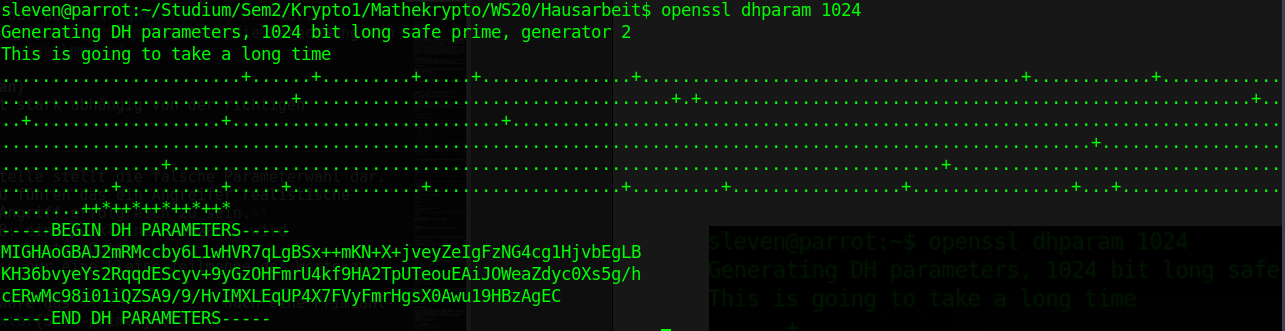
\includegraphics[scale=0.41]{dh}     
\end{figure}
\newpage
\subsection{Man in the Middle} 

Grundprinzip dieser Angriffsvariante ist es gegenüber B vorzutäuschen man sei A und gegenüber A vorzutäuschen man sei B.
Ziel ist es Kenntnis des Shared Secrets zu erhalten!\\
Konkret heißt das folgendes:\\
'Alice' wählt wie gewohnt ein geheimes Element $a$ und berechnet $g^a$ das Sie an 'Bob' senden will!
Der Abhöhrer 'Sean' fängt diese Nachricht ab, gibt vor Bob zu sein und generiert selber einen private key $S$ mit dem er $g^s$ berechnet und dies an Alice sendet! Die Parteien führen also ein kompletten Key exchance aus der als Shared Secret $g^(as)$ resultiert.\footnote{Vorlesungsfolien}\\
Nun sendet Sean $g^s$ an Bob und erhält von ihm $g^b$ was wieder in einem shared secret $g^sbs$ endet.\\
Sean hat also beide shared secrets und kann somit jeglichen Datenaustausch mithören oder verändern!\footnote{\cite{10.1007/978-3-540-39927-8_28}}\\



\begin{center}
 Alice  ($g^a \mod p$ $)  \rightarrow$ \hspace{2cm}  Sean \hspace{4cm} Bob\\
 Alice   \hspace{3.9cm}  Sean ($g^s \mod p$ $) \rightarrow$ \hspace{2.1cm} Bob\\
 Alice   \hspace{3.9cm}  Sean \hspace{2.2cm} $\leftarrow$ ($g^b \mod p$) Bob\\
 Alice   \hspace{2.2cm}$\leftarrow$ ($g^s \mod p$)  Sean \hspace{4.1cm}  Bob\\
 

 
 
\end{center}

In einem schlecht automatisierten Verfahren würde der vorliegende Fall nicht auffallen.\\
\textbf{Lösung} für dieses Problem stellt die Variante 'Authenticated Diffie-Hellman' dar!\\
Diese integriegt gegenseitige Authentisierung mittels digitaler Signaturen. Hierbei muss sich Alice den Public Key (RSA) bon Bob besorge, um dessen Signatur prüfen zu können. Gleichsam benötigt Bob jenen von Alice!
\begin{center}
 Alice ($g^a \mod p$ , $\mathbb{\text{SIG}}_{Alice}$)  \hspace{3cm} $\rightarrow$ \hspace{2cm} Bob\\
 Alice   \hspace{3.4cm} $\leftarrow$ \hspace{2cm}($g^b \mod p$ , $\mathbb{\text{SIG}}_{Bob}$) Bob
\end{center}



\newpage
\subsection{Discrete Logarithm Problem}
Dieser Angriff zielt direkt auf das Mathematische Grundprinzip ab.\\
$\Rightarrow$
Versuche, mit Kenntnis der Parameter $p$, $g$, sowie mit $g^a \mod p$ den Exponenten $a$ zu
ermitteln.\\
 Die Erfolgschancen hierbei hängen  stark von den gewählten Parametern ab. Sind diese richtig gewählt, sprich große 'safe Primes' wird es praktisch unmöglich eine erfolgreiche Berechnung durchzuführen.\\
Für ein weiteres Beispiel folgendes Szenario mit bewusst kleinen Zahlen:\\
Angenommen beide Gesprächspartner einigen sich auf das Element $\mathbb{Z}_{11}$*. Für ein Angreifer der über ein unsicheren Kanal abhört stellt sich nun folgende Frage:\\
\begin{center}
 $2^a \equiv 3 \mod 11$
\end{center}
Ist hier die Antwort $3$ selbst ohne Taschenrechner zu ermitteln so wird bei hohen Primzahlen die Berechnungsdauer derart unpraktikabel dass man von praktisch unmöglichen Erfolgschancen sprechen kann!\footnote{\cite{10.1007/11761679_1}}
\\
\newline
\subsection{Computational Diffie-Hellman Problem CDH}
Das CDH ist eng verwand mit den DLP.\\
$\Rightarrow$ Hiebei gilt es mit Kenntnis der Parameter $p$, $g$, sowie mit $g^a \mod p$ und $g^b \mod p$ den Wert $g^(ab) \mod p$ zu ermitteln.\\
Gilt durch die Ähnlichkeit der beiden wenn DLP gelöst $\Rightarrow$ CDH gelöst?\\

Falls jemand in der Lage ist, aus $g^a \mod p$ den Exponenten $a$ zu ermitteln, beziehungsweiße aus $g^b \mod p$ den Exponenten $b$ zu ermitteln so hat er das 'Diskrete Logarithm Problem' gelöst.\footnote{Vorlesungsfolien}\\
Nun stellt sich die Frage in wie weit das zur Lösungsfindung des  CDH beiträgt!\\
Hat man Kenntnis von $a$ und $b$ ist es trivial den Wert $g^(ab) \mod p$ zu berechnen. Somit kann man Aussgenlogisch festhalten
\begin{center}
 DLP lösbar $\Rightarrow$ CDH lösbar\\
 CDH nicht lösbar $\Rightarrow$ DLP nicht lösbar
\end{center}
Die umgekehrte Richtung ist jedoch noch immer ungelöst. Bislang konnte niemand zeigen,
ob gilt: CDH lösbar $\Rightarrow$ DLP lösbar.\footnote{\cite{10.1007/978-3-540-39927-8_28}}

\newpage
\subsection{Decisional Diffie-Hellman Problem}

Versuche mit Kenntnis der Parameter $p$ und $g$ sowie mit $g^a \mod p$  und $g^b \mod p$ die folgende Frage zu beantworten:\\
Angenommen man erhält die beiden Werte $x = g^(ab) \mod p$ sowie $y = g^c \mod p$ für irgendein $c$. Entscheide, welcher der beiden Werte das Shared Secret $g^(ab) \mod p$ darstellt!
Auch hier kann man die Aussagenlogik weiterführen.\footnote{\cite{10.1007/BFb0054851}}\\
\begin{center}
 CDH lösbar $\Rightarrow$ DDH lösbar
 
\end{center}


\section{Conclusion}
Diffie-Hellman stellt nun seit mehr als 40 Jahren zusammen mit RSA den Standart für Public-Key Kryptografie dar. Zwar gibt es schon heutzutage theoretische Angriffsmodelle die DH knacken können, jedoch sind die meisten erfolgreichen Angriffe auf falsche konfiguration bzw. Benutzung des Protokolls zurückzuführen, nicht aber auf die Mathematische Sicherheit. Die Frage ist, ob dies in Zukunft so bleiben wird. Schaut man sich die Entwicklung von Quanten Computern der letzten 10 Jahre an, stellt man fest das diese keine theoretischen Konzepte mehr sind, sondern in absehbarer Zeit wirklichkeit werden könnten! Jetzige Umsetzungen, wie der von Google sind sehr speziallisierte ausführungen und noch nicht in der Lage Kryptografischen Methoden gefährlich zu werden. Jedoch zeigt dies das es nicht mehr lange dauern wird. Es gibt schon jetzt Überlegegungen DH als Standart Abzulösen durch Umsetzungen wie ECDH 
Elliptic curve Diffie Hellman. Letzendlich ist das ganze abhängig davon wie schnell es gelingen wird Quenten Computing anwendbar zu machen. Wird dies der Fall sei, müssten allerdings komlett neue Konzepte entwickelt werden, und Diffie Hellman würde keine Rolle mehr spielen!\footnote{Vorlesungsfolien}
\newpage
\section{Quellen}
\printbibliography
https://cryptography.fandom.com/wiki/Diffie-Hellman-key-exchange
\end{document}
